\documentclass[
  sigplan,
  10pt,
  anonymous,
  review,
  ]{acmart}
\settopmatter{printfolios=true,printccs=false,printacmref=false}

\usepackage[british]{babel}

\usepackage[capitalise]{cleveref}

\usepackage{mathpartir}

% Record brackets
\usepackage{stmaryrd}

\usepackage{xcolor}

\usepackage{tikz}
\usetikzlibrary{shapes,positioning,patterns,patterns.meta}
\usepackage{pgfplots}
\pgfdeclarelayer{background}
\pgfdeclarelayer{foreground}
\pgfsetlayers{background,main,foreground}

\usepackage{enumitem}

\usepackage{array}
\usepackage{multirow}

\usepackage{listings}
\definecolor{isarblue}{HTML}{006699}
\definecolor{isargreen}{HTML}{009966}
\lstdefinelanguage{isabelle}{%
    keywords=[1]{type_synonym,typedef,datatype,fun,function,abbreviation,definition,proof,lemma,theorem,corollary,inductive,record},
    keywordstyle=[1]\bfseries\color{isarblue},
    keywords=[2]{where,assumes,shows,and,fixes,defines},
    keywordstyle=[2]\bfseries\color{isargreen},
    keywords=[3]{if,then,else,case,of,SOME,let,in,O},
    keywordstyle=[3]\color{isarblue},
}
\lstset{%
  language=isabelle,
  escapeinside={&}{&},
  columns=\lst@ifdisplaystyle{fullflexible}\else{fixed}\fi,,
  extendedchars,
  basewidth={0.5em,0.45em},
  basicstyle=\ttfamily,
  mathescape,
}
\makeatletter
\lst@AddToHook{OnEmptyLine}{\vspace{-0.4\baselineskip}}
\makeatother
\newcommand{\lstinlinew}[2][]{\lstinline[#1]{#2}}
% This is a hack to allow escaping inside lstinline (https://tex.stackexchange.com/questions/43526/escaping-in-lstinline)
\usepackage{etoolbox}
\makeatletter
\patchcmd{\lsthk@TextStyle}{\let\lst@DefEsc\@empty}{}{}{\errmessage{failed to patch}}
\makeatother

\usepackage{calc}

\newcommand{\textover}[3][l]{%
 % #1 is the alignment, default l
 % #2 is the text to be printed
 % #3 is the text for setting the width
 \makebox[\widthof{#3}][#1]{#2}%
}

\hyphenation{Isa-belle}

% For arXiv: LuaLatex on Arxiv: https://tex.stackexchange.com/questions/372154/lualatex-how-to-produce-pdf-acceptable-by-arxiv 
%\hypersetup{%
%  pdfcreator = {},
%  pdfproducer = {}
%}
%\pdfvariable suppressoptionalinfo \numexpr 1+2+4+8+16+32+64+128+256+512 \relax

% For arXiv: Remove copyright information
% \setcopyright{none}
% \renewcommand\footnotetextcopyrightpermission[1]{}


\usepackage{todonotes}

% Autoref names
\renewcommand{\sectionautorefname}{Section}
\renewcommand{\subsectionautorefname}{Section}

% Acronyms
\usepackage[acronym]{glossaries}
\newacronym{adt}{ADT}{abstract data type}
\newacronym{uf}{UF}{Union-Find}
\newacronym{ufe}{UFE}{Union-Find-Explain}
\newacronym{lca}{LCA}{lowest common ancestor}
\newacronym{afp}{AFP}{Archive of Formal Proofs}
\newacronym{smt}{SMT}{Satisfiability Modulu Theories}


% Notation
\newcommand{\TransP}{\bigtriangledown}
\newcommand{\NewestL}[3]{(#2 $\upharpoonleft$ #3)$_\text{#1}$}
\newcommand{\NewestR}[3]{(#2 $\upharpoonright$ #3)$_\text{#1}$}
\newcommand{\opunion}{union}
\newcommand{\opfind}{find}
\newcommand{\opexplain}{explain}

\begin{document}

% For arXiv: Remove conference/author in the header
% \pagestyle{plain}

\setcounter{tocdepth}{1}

\title{Simplified and Verified: A Second Look at a Proof-Producing Union-Find Algorithm}
\author{Lukas Stevens}
\orcid{0000-0003-0222-6858}
\affiliation{%
  \institution{Technical University of Munich}
  \department{Department of Informatics}
  \streetaddress{Boltzmannstr. 3}
  \city{Garching}
  \postcode{85748}
  \country{Germany}
}
\email{lukas.stevens@in.tum.de}

\author{Rebecca Ghidini}
\orcid{0009-0009-8117-2659}
\affiliation{%
  \institution{Technical University of Munich}
  \department{Department of Informatics}
  \streetaddress{Boltzmannstr. 3}
  \city{Garching}
  \postcode{85748}
  \country{Germany}
}
\email{rebecca.ghidini@tum.de}

\begin{abstract}
  TODO
\end{abstract}

\maketitle

\section{Introduction}
The \acrfull{uf} data structure maintains the equivalence closure of a relation, where the relation is given as a sequence of pairs or, in terms of the \acrshort{uf} data structure, \opunion operations.
It is fundamental to efficiently implement well-known graph algorithms such as \citeauthor{mst}'s~\cite{mst} minimum spanning tree algorithm. 
There it tracks which vertices belong to the same connected component and are, in that sense, equivalent.
Beyond graph algorithms, its applicability extends to the domain of theorem proving as it routinely forms the basis of congruence closure algorithms, which are widely used by \acrfull{smt} solvers.
In order to increase their trustworthiness, current \acrshort{smt} solvers such as CVC5~\cite{cvc5}, E~\cite{eprover}, Vampire~\cite{vampire}, VeriT~\cite{verit}, and Z3~\cite{z3_proofs} are able to output detailed proofs if they determine their input formula to be unsatisfiable.

\begin{itemize}
  \item Based on \cite{congcl_proofs}
  \item Especially in the context of theorem proving certificates are useful
  \item Maybe cite order paper
\end{itemize}

\subsection{Contributions}
\begin{itemize}
  \item Formalisation of \acrshort{ufe} data structure
  \item Reduction of the complex recursion scheme to a simpler one that produces the same output
  \item Proof of soundness, completeness, and termination
  \item Abstract formalisation of union-find and union-find with size information hiding implementation details behind type definition
  \item Refinement of the \acrshort{ufe} to Imperative HOL to be able to export efficient code
\end{itemize}
\todo[inline]{We only show proof sketches, details in the formalisation}

\subsection{Related Work}
\begin{itemize}
  \item Union-Find as forest and union-by-size \cite{uf_by_size}
  \item Path compression \cite{uf_compress}
  \item Analysis of the run-time: $\mathcal{O}(n + m \alpha(m + n, n))$ for a sequence of at most $n - 1$ unions and $m$ finds \cite{uf_ub_improved}
  \item In Coq \cite{uf_coq} with time \cite{uf_coq_time}
  \item In Isabelle \cite{uf_isabelle} with time \cite{uf_isabelle} more recently viewed algebraically \cite{uf_isabelle_algebraic}.
\end{itemize}

\subsection{Notation}
Isabelle/HOL~\cite{isabelle} conforms to everyday mathematical notation for the most part.
We establish notation and in particular some essential data types together with their primitive operations that are specific to Isabelle/HOL.

We write \lstinline!t :: 'a! to specify that the term \lstinline!t! has the type \lstinline!'a! and \lstinline!'a $\Rightarrow$ 'b! for the space of total functions from type \lstinline!'a! to type \lstinline!'b!.

Sets with elements of type \lstinline!'a! have the type \lstinline!'a set!.
The cardinality of a set \lstinline!A! is denoted by \lstinline!card A! and the image of \lstinline!A! under \lstinline!f! by \lstinline!f ` A!.

We use \lstinline!'a list! to describe the type of lists, which are constructed using the empty list \lstinline![]! constructor or the infix cons constructor \lstinline!#!, and are appended with the infix operator \lstinline!@!.
The function \lstinline!set! converts a list into a set.
\todo[inline]{Indexing operator}
\todo[inline]{Relation type synonym, Field of a relation}
\todo[inline]{Record notation}
\todo[inline]{Order on options}
\todo[inline]{Locale notation}
\todo[inline]{Lemma numbering}

We remark that $\longleftrightarrow$ is equivalent to \lstinline!$=$! on the type of Booleans \lstinline!bool! and \lstinline!$\equiv$! is definitional equality of the meta-logic of Isabelle/HOL, which is called Isabelle/Pure.
Meta-implication is denoted by \lstinline!$\Longrightarrow$! and a chain of implications
\begin{lstlisting}
  A$_\text{1}$ $\Longrightarrow$ $\cdots$ $\Longrightarrow$ A$_\text{k}$ $\Longrightarrow$ C
\end{lstlisting}
can be abbreviated by 
\begin{lstlisting}
  $\llbracket$ A$_\text{1}$;$\,\ldots\,$;A$_\text{k}$ $\rrbracket$ $\Longrightarrow$ C.
\end{lstlisting}

\section{Basic Union-Find}
\subsection{Background\label{sec:uf_background}}
Given a set of $n$ elements $A = \{a_1, \ldots, a_n\}$, the \acrfull{uf} data structure keeps track of a partition of $A$ into disjoint sets $A_1, \ldots, A_k$, i.e.\ $A = A_1 \uplus \cdots \uplus A_k$.

We initialise the data structure by partitioning $A$ into singleton sets of elements,
so we have that $A = \{a_1\} \uplus \cdots \uplus \{a_n\}$.
Those sets are merged by subsequent \lstinline!union! operations\todo{use italics for union operation?} where \lstinline!union $a_i$ $a_j$! merges the set containing $a_i$ with the one that contains $a_j$.
Each set in the partition contains one particular element that serves as its representative.
We will denote the representative of an element $a$ in the \acrshort{uf} data structure $l$ as \lstinline!rep_of $l$ $a$!.
Accordingly, two elements have the same representative exactly when they belong to the same set in the partition.
For any element $a_i$, the \lstinline!find! operation just returns its representative \lstinline!rep_of $l$ $a_i$!.

One application of this algorithm is to maintain the equivalence closure of equations, which is the partial equivalence relation formed by those equations.
To this end, we initialize the \acrshort{uf} data structure with $n$ elements for a given set of variables $v_1, \ldots, v_n$ and perform a \lstinline!union! between $v_i$ and $v_j$ for each equation $v_i = v_j$.
This results in a partition of the variables into equivalence classes.

The data structure can be implemented as a forest of rooted trees where each tree represents an equivalence class.
The edges of the trees are directed towards their root, which is the representative of the corresponding equivalence class.
To keep this invariant, we initialise the forest with $n$ nodes but without any edges and for every \lstinline!union! of $a_i$ and $a_j$ we add a directed edge from \lstinline!rep_of $l$ $a_i$! to \lstinline!rep_of $l$ $a_j$! to the forest.

We encode such a forest as a list $l$ of length $n$, where at each index $i$ of the list, we save the parent of the element $i$.
Therefore, we denote the parent of an element $a$ with \lstinline|$l$ ! $a$|.
If $a$ is a root and thus does not have a parent, then the list contains the element $a$ itself at the index $a$, i.e., \lstinline|$l$ ! $a$ = $a$|.

\subsection{In Isabelle/HOL\label{sec:uf_hol}}
The \acrshort{uf} algorithm is formalised in Isabelle/HOL by \citeauthor{uf_isabelle}~\cite{uf_isabelle}.
The code can be found in an entry~\cite{uf_isabelle_afp} of the \acrfull{afp}.\footnote{The code is in the theory file \texttt{Examples/Union\_Find.thy}.}
Later, \citeauthor{uf_isabelle}~\cite{uf_isabelle} also formalised the running time.\todo{Check citations}

The formalisation defines a function \lstinline|rep_of|, which, as described in the previous section, follows the parent pointers until we arrive the root, where the parent pointer is self-referential.
\begin{lstlisting}[columns=fullflexible]
function rep_of :: nat list $\Rightarrow$ nat $\Rightarrow$ nat where
rep_of l a =
  if l ! a = a then a else rep_of l (l ! a)
\end{lstlisting}
Looking closely at this definition, we see that this function is only well-defined for some inputs \lstinline|l| and \lstinline|a|:
for every element \lstinline|a < length l|, its parent must be in the list, i.e.\ we must have \lstinline|l ! a < length l|, and the parent pointers must be cycle-free in order for the function to terminate.
Functions in Isabelle/HOL must be total, so the \lstinline|function| command introduces a constant
\begin{lstlisting}
rep_of_dom :: (nat list $\times$ nat) $\Rightarrow$ bool  
\end{lstlisting}
that characterises the inputs for which \lstinline|rep_of| terminates.
Then, it adds \lstinline|rep_of_dom (l, a)| as a premise to the defining equation of \lstinline|rep_of|. 
The intuition above is cast into a predicate \lstinline|ufa_invar| that defines such well-formed lists \lstinline|l|.
\begin{lstlisting}
definition ufa_invar l = $\forall$a < length l.
  rep_of_dom (l, a) $\land$ l ! a < length l
\end{lstlisting}
Building on this formalisation, we encapsulate this \acrshort{uf} data structure into an \acrfull{adt} \lstinline|ufa| by defining
\begin{lstlisting}
typedef ufa = {uf. ufa_invar uf}
\end{lstlisting}
By lifting operations on the underlying list to the \acrshort{adt} using Isabelle's lifting infrastructure~\cite{lifting_transfer}, we obtain the operations
\begin{itemize}
  \item \lstinline!ufa_$\alpha$ :: ufa $\Rightarrow$ nat rel!,
  \item \lstinline!ufa_rep_of :: ufa $\Rightarrow$ nat $\Rightarrow$ nat!, and
  \item \lstinline!ufa_union :: ufa $\Rightarrow$ nat $\Rightarrow$ nat $\Rightarrow$ ufa!,
\end{itemize}
where \lstinline!nat rel = (nat $\times$ nat) set!.
The intended meaning of these operations is the following:
\begin{itemize}
  \item \lstinline!ufa_$\alpha$ uf! is the partial equivalence relation represented by \lstinline!uf!,
  \item \lstinline!ufa_rep_of uf x! is the representative of the equivalence class that \lstinline!x! belongs to, and
  \item \lstinline!ufa_union uf x y! returns a \acrshort{uf} data structure where the equivalence classes of \lstinline!x! and \lstinline!y! are merged.
    This is implemented by updating the underlying list at index \lstinline!rep_of l x! to \lstinline|rep_of l y|.
\end{itemize}
More rigorously, the above operations fulfil the following properties:
\begin{lstlisting}
lemma ufa_rep_of uf x = ufa_rep_of uf y $\longleftrightarrow$
  (x, y) $\in$ ufa_$\alpha$ uf

lemma ufa_$\alpha$ (ufa_union uf x y) =
  per_union (ufa_$\alpha$ uf) x y
\end{lstlisting}
where \lstinline!per_union R x y! is defined as the equivalence relation that results from merging the respective equivalence classes in the relation \lstinline|R| that \lstinline!x! and \lstinline!y! belong to.

But what happens if \lstinline!x! or \lstinline!y! is not an element of the partial equivalence relation \lstinline|R|?
In that case, the equivalence relation is unchanged, which means that \lstinline|per_union R x y = R|.
This, however, can be seen as a misuse of the \acrshort{uf} data structure, since we initialise it with a fixed set of elements \lstinline|A| and expect the user to only work with these elements.
Therefore, we introduce the following definitions that characterise valid union(s) with regard to this initial set.
\begin{lstlisting}
definition valid_union uf a b =
  a $\in$ Field (ufa_$\alpha$ uf) $\land$ b $\in$ Field (ufa_$\alpha$ uf)
definition valid_unions uf us =
  $\forall$(x, y) $\in$ set us. valid_union uf x y
\end{lstlisting}

\section{Simple Certifying Union-Find Algorithm}
\begin{figure}
  \begin{gather*}
    \inferrule*[right=Assm]{\hbox{\lstinline|i < length us|} \\ \hbox{\lstinline|us ! i = (x, y)|}}{\hbox{\lstinline|us $\ \vdash_=\ $ AssmP i : (x, y)|}} \\[0.5em]
    \inferrule*[right=Refl]{ }{\hbox{\lstinline|us $\ \vdash_=\ $ ReflP x : (x, x)|}} \\[0.5em]
    \inferrule*[right=Sym]{\hbox{\lstinline|us $\ \vdash_=\ $ p : (x, y)|}}{\hbox{\lstinline|us $\ \vdash_=\ $ SymP p : (y, x)|}} \\[0.5em]
    \inferrule*[right=Trans]{\hbox{\lstinline|us $\ \vdash_=\ $ p1 : (x, y)|} \\ \hbox{\lstinline|us $\ \vdash_=\ $ p2 (y, z)|}}{\hbox{\lstinline|us $\ \vdash_=\ $ p1 $\ \TransP\ $ p2 : (x, z)|}}
  \end{gather*}
  \caption{The data type \lstinline|eq_prf| of certificates and its corresponding system of inference rules $\vdash_=$.\label{fig:eq_prf}}
\end{figure}
\todo[inline]{Use equivalence instead of equality, Use equivalence operator instead of pairs, Maybe use cong symbol}
Building on the \acrshort{uf} \acrshort{adt} from the previous section, we now develop a simple \lstinline|explain| operation that,
for a given list of equations \lstinline|us|, takes two elements \lstinline|x| and \lstinline|y| and produces a certificate that \lstinline|x = y| modulo \lstinline|us|.
The certificate is given in terms of a data type \lstinline|eq_prf| with its corresponding system $\vdash_=$ of inference rules as seen in \autoref{fig:eq_prf}.
As expected, we have inference rules that utilise the reflexivity, symmetry, and transitivity of equality as well as an assumption rule.
To improve readability, we use the infix operator $\bigtriangledown$ to denote the proof term for transitivity.

We remark that one can not prove disequality with this proof system.
In that sense, we are working with an open-world assumption. 

We prove that $\vdash_=$ is sound and complete with respect to the equivalence relation induced by \lstinline|us|, i.e.\ the equivalence closure of \lstinline|us|.
In Isabelle, we define\todo{Introduce inverse and rtrancl?}
\begin{lstlisting}
definition symcl r = r $\cup$ r$^{-1}$
definition equivcl r = (symcl r)$^*$
\end{lstlisting}
and prove
\begin{lstlisting}
lemma $\vdash_=$_sound:
assumes as $\vdash_=$ p : (x, y)
shows (x, y) $\in$ equivcl (set as)

lemma $\vdash_=$_complete:
assumes (x, y) $\in$ equivcl (set as)
shows $\exists$p. as $\vdash_=$ p : (x, y)
\end{lstlisting}

\begin{figure*}
  \centering
  \begin{lstlisting}
function explain :: (nat $\times$ nat) list $\Rightarrow$ nat $\Rightarrow$ nat $\Rightarrow$ nat eq_prf where
  explain [] x _ = ReflP x
| explain (us @ [(a, b)]) x y =
    let uf = ufa_unions uf_init us; a_b_P = AssmP (length us)
    in if ufa_rep_of uf x = ufa_rep_of uf y then explain us x y
      else if ufa_rep_of uf x = ufa_rep_of uf a then explain us x a $\TransP$ a_b_P $\TransP$ explain us y b
      else explain us x b $\TransP$ SymP a_b_P $\TransP$ explain us a y

definition explain_partial us x y =
  if (x, y) $\in$ equivcl (set us) then Some (explain us x y) else None
  \end{lstlisting}
  \caption{A simple implementation of the \lstinline|explain| operation. It operates on an arbitrary initial \acrshort{uf} data structure \lstinline|uf_init|.\label{fig:explain}}
\end{figure*}
\todo[inline]{termination of \lstinline|explain|}
Although \lstinline|explain| takes a list of equations \lstinline|us|, its implementation actually works with an instance \lstinline|uf| of the \acrshort{uf} \acrshort{adt} that results from applying \lstinline|us| as unions to an initial \acrshort{uf} data structure \lstinline|uf_init|.
Accordingly, we define
\begin{lstlisting}
definition ufa_unions =
  foldl ($\lambda$uf (x, y). ufa_union uf x y)
\end{lstlisting}
so we have \lstinline|uf = ufa_unions uf_init us| in terms of the constants above.

At last, we are ready to implement the \lstinline|explain| operation as depicted in \autoref{fig:explain}.
The algorithm works with the assumption that the given elements \lstinline|x| and \lstinline|y| are equal modulo \lstinline|us|.
Furthermore, we assume that each element of the initial data structure \lstinline|uf_init| is equal to itself
and that \lstinline|us| are valid unions with respect to \lstinline|uf_init|.
In formulae, we assume
\begin{itemize}
  \item \lstinline|ufa_$\alpha$ uf_init $\subseteq$ Id|, and
  \item \lstinline|valid_unions uf_init us|
\end{itemize}
in the remainder of this section.

If the list of unions is empty, then \lstinline|x| and \lstinline|y| must actually be equal which we certify with \lstinline|ReflP x|.

Otherwise, the list of unions must be equal to \lstinline|us @ [(a, b)]| for some \lstinline|us|, \lstinline|a|, and \lstinline|b|.
We distinguish between two cases:
\begin{itemize}
  \item The elements \lstinline|x| and \lstinline|y| are already equal modulo \lstinline|us|, so we proceed recursively with \lstinline|us|.
  \item In the case that the equation \lstinline|a = b| is necessary for \lstinline|x = y| to hold, we either have \lstinline|x = a| and \lstinline|b = y| or \lstinline|x = b| and \lstinline|a = y| modulo \lstinline|us|.
    Assuming that the former holds --- the other case is symmetric --- we recursively construct the certificates for \lstinline|x = a| and \lstinline|b = y|.
    Together with the assumption that \lstinline|a = b|, we obtain \lstinline|x = y| by transitivity.
\end{itemize}

We condense the above intuition into the completeness theorem below.
\begin{lstlisting}
theorem explain_complete:
assumes (x, y) $\in$ equivcl (set us)
shows us $\vdash_=$ explain uf_init us x y : (x, y)
\end{lstlisting}

The \lstinline|explain| function is not sound, though.
This is because it always returns a certificate, even if \lstinline|x| and \lstinline|y| are not equal modulo \lstinline|us|.
To account for this case, we wrap \lstinline|explain| into a partial function \lstinline|explain_partial| (cf.\ \autoref{fig:explain}) that fails if \lstinline|x = y| is not provable.
Soundness and completeness can then be lifted from the soundness of $\vdash_=$ and the completeness of \lstinline|explain|, respectively.
At first glance, it might seem vacuous to define \lstinline|explain_partial| using \lstinline|equivcl|;
however, \lstinline|equivcl| can actually be implemented using \acrshort{uf} operations as the following lemma demonstrates.
\begin{lstlisting}
lemma
defines uf = ufa_unions uf_init us
shows (x, y) $\in$ equivcl (set us) $\leftrightarrow$ x = y $\lor$
  x $\in$ Field (ufa_$\alpha$ uf) $\land$ y $\in$ Field (ufa_$\alpha$ uf) $\land$
  ufa_rep_of uf x = ufa_rep_of uf y
\end{lstlisting}
\todo[inline]{Improve explanation above? Segue?}

\section{Efficient Certifying Union-Find Algorithm}
In the previous section, we developed a simple certifying \acrfull{ufe} data structure whose \lstinline|explain| operation iterates through a list of equalities,
identifying which of them are necessary in order to prove that the inputs are equal.
Nevertheless, iterating through all equalities seems inefficient and indeed \citeauthor{congcl_proofs}~\cite{congcl_proofs} propose a more focused approach.
Specifically, they use a \acrshort{uf} data structure represented as forest of rooted trees as described in \autoref{sec:uf_background}.
They modify the data structure such that, for each union between \lstinline|a| and \lstinline|b|, the newly added edge gets annotated with \lstinline|(a, b)|.\todo{Direction of union! Explain sides of the union!}
To understand why this allows for a more efficient implementation of the explain operation, suppose that we want to certify that \lstinline|x| is equal to \lstinline|y|.
Clearly, only the edges of the subtree rooted at the \acrfull{lca} of \lstinline|x| and \lstinline|y|, as illustrated in \autoref{fig:explain'_abs}, are relevant to explain why \lstinline|x| is equal to \lstinline|y|.
Furthermore, let \lstinline|(a, b)| be the most recent union on either of the paths between the \acrshort{lca} and \lstinline|x| and \lstinline|y|, respectively.
\todo[inline]{Intuition: path from x to y}
Here, we assume w.l.o.g.\ that \lstinline|(a, b)| is on the path to \lstinline|x|.
The corresponding edge separates the tree rooted at the \acrshort{lca} into two subtrees as indicated by the patterns,  one containing \lstinline|a| and the other one \lstinline|b|.
Moreover, the paths from the \acrshort{lca} can't overlap, so \lstinline|x| and \lstinline|y| also belong to different subtrees.
Ultimately, to certify the equality of \lstinline|x| and \lstinline|y|, we recursively prove that \lstinline|x| is equal to \lstinline|a| and \lstinline|y| to \lstinline|b|.
Then, we put everything together using transitivity and the equality of \lstinline|a| and \lstinline|b|.
This terminates since \lstinline|(a, b)| is the most recent union and we only consider less recent unions in the recursive steps.
All in all, this gives a $\mathcal{O}(k \log n)$ explain operation where $k$ is the number of unions required for an explanation~\cite{congcl_proofs}.
\todo[inline]{Running time of naive algorithm}
\begin{figure}
  \centering
  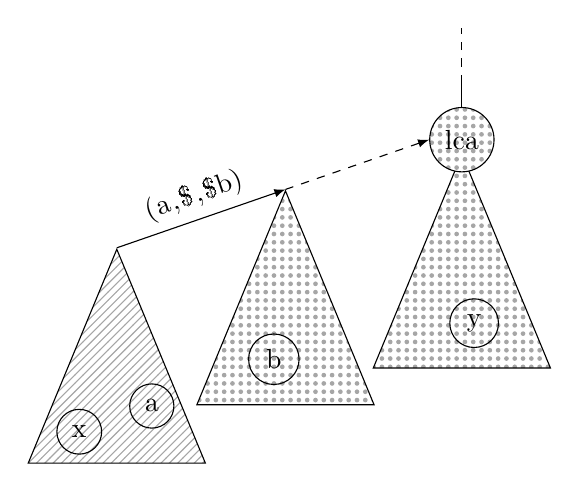
\begin{tikzpicture}[
    >=latex, node distance=0.5cm,
    aside/.append style={pattern=north east lines, pattern color=gray!70},
    bside/.append style={pattern={Dots[radius=0.85pt]}, pattern color=gray!70}
    ]
    \node[draw, circle, preaction={fill, white}, style=bside] (lca) {\acrshort{lca}};
    \begin{pgfonlayer}{background}
      \begin{scope}[shape=isosceles triangle, shape border rotate=90, minimum height=2cm, minimum width=2.25cm]
        \node[draw, anchor=north, below left=2.5cm and 3.5cm of lca.south west, aside] (l) {};
        \path (l.north) -- node[pos=0.54, draw, anchor=north, bside] (m) {} (lca.west);
        \node[draw, anchor=north, yshift=0.25cm, bside] (r) at (lca.south) {};
      \end{scope}
    \end{pgfonlayer}

    \node[draw, circle, above right=0.2cm and 0.05cm of l.south west] (x) {\lstinline|x|};
    \node[draw, circle, left=0.1cm of l.east] (a) {\lstinline|a|};
    \node[draw, circle, above left=of r.south east] (y) {\lstinline|y|};
    \node[draw, circle, above right=of m.south west] (b) {\lstinline|b|};
    
    \draw[->] (l.north) -- node[above, sloped] {\lstinline|(a,$\,$b)|} (m.north);
    \draw[->, dashed] (m.north) -- (lca.west);
    \draw[solid] (lca.north) -- ++(0,0.3);
    \draw[dashed] (lca.north) ++(0,0.3) -- ++(0,0.7);
  \end{tikzpicture}
  \caption{High-level workings of the \lstinline|explain'| function.\label{fig:explain'_abs}}
\end{figure}

\subsection{Implementation}
We implement this \acrshort{ufe} data structure as a record type \lstinline|ufe_ds|.
For some fixed instance \lstinline|ufe_ds| of this type, the purpose of the record members is as follows:
\todo[inline]{Introduce \lstinline|ufa_parent_of|, explain abstraction leakage.}
\begin{itemize}
  \item The list \lstinline|unions ufe_ds :: (nat $\times$ nat) list| contains the input equalities.
  \item The \acrshort{ufe} data structure \lstinline|uf_ds ufe_ds :: ufa| maintains the equivalence closure of the input equalities or, put differently, it is the result of applying \lstinline|unions ufe_ds| to an initial union find data structure.
    We require this to be a forest of rooted trees as introduced in \autoref{sec:uf_background}.
  \item The partial function \lstinline|au_ds ufe_ds :: nat $\Rightarrow$ nat option| associates an unique equality with each edge in the forest by indexing into \lstinline|unions ufe_ds|.
    In other words, there exists an \lstinline|i| such that \lstinline|au_ds ufe_ds x = Some i| if \lstinline|x| has a parent in the forest.
    The associated union of the edge from \lstinline|x| to its parent is then \lstinline|unions ufe_ds ! i|.
\end{itemize}
For succinctness, we lift the operations \lstinline|ufa_rep_of|, \lstinline|ufa_parent_of|, and \lstinline|ufa_$\alpha$| from the record member \lstinline|uf_ds| to the record type \lstinline|ufe_ds|.
The lifted operations use the prefix \lstinline|ufe| instead of \lstinline|ufa|, so \lstinline|ufa_rep_of| is lifted to \lstinline|ufe_rep_of|, for example.

Similarly, we obtain the initial \acrshort{ufe} data structure by lifting \lstinline|ufa_init| while leaving the other two members empty as the following definition shows.
\todo[inline]{Introduce \lstinline|ufa_init|. Say that this is the init operation?}
\begin{lstlisting}
definition ufe_init :: nat $\Rightarrow$ ufe_ds where
  ufe_init n = $\llparenthesis$ uf_ds = ufa_init n,
    au_ds = ($\lambda$_. None), unions = [] $\rrparenthesis$
\end{lstlisting}

\subsubsection{Union}
Continuing with the union operation, we lift \lstinline|ufa_union| to the \acrshort{ufe} data structure.
For a union operation between \lstinline|x| and \lstinline|y|, we add \lstinline|(x, y)| to the list of unions and update the associated union of the representative of \lstinline|x| to \lstinline|(x, y)|.
We need to use the representative here because \lstinline|ufa_union| adds an edge from the representative of \lstinline|x| to that of \lstinline|y|.
As with the \acrshort{uf} data structure, we also define a function that applies a list of unions in consecutive order.
\begin{lstlisting}
fun ufe_union :: ufe_ds $\Rightarrow$ nat $\Rightarrow$ nat
              $\Rightarrow$ ufe_ds where
  ufe_union $\llparenthesis$ uf_ds = uf
            , au_ds = au, unions = u $\rrparenthesis$ x y =
    $\llparenthesis$ uf_ds = ufa_union uf x y
    , au_ds = au(ufa_rep_of uf x $\mapsto$ length u)
    , unions = u @ [(x, y)] $\rrparenthesis$

definition ufe_unions = 
  foldl ($\lambda$ufe_ds (x, y). ufe_union ufe_ds x y)
\end{lstlisting}
The definition of \lstinline|ufe_union| comes with a caveat:
specifically, it only makes sense to update the (associated) unions if the union in question actually introduces a new edge in the \acrshort{uf} data structure.
In other words, the representatives of \lstinline|x| and \lstinline|y| of the union \lstinline|(x, y)| must not be equal.
We call such a union \emph{effective} with respect to a given \acrshort{uf} data structure.
This notion extends to lists of unions by checking if each consecutive union is effective with respect to the data structure that results from applying the preceeding unions.
\begin{lstlisting}
definition eff_union uf a b =
  valid_union uf a b $\land$
  ufa_rep_of uf a $\neq$ ufa_rep_of uf b

fun eff_unions where
  eff_unions uf [] $\leftrightarrow$ True
| eff_unions uf ((a, b) # us) $\leftrightarrow$
    eff_union uf a b $\land$
    eff_unions (ufa_union uf a b) us
\end{lstlisting}

\subsubsection{Well-formed \acrshort{ufe} data structures}
In the previous sections, we have introduced the prerequisites for creating \acrshort{ufe} data structures,
namely a way to initialise the data structure and the union operation.
We refer to data structures created in this way as well-formed.
In order to characterise well-formedness, we employ a feature of Isabelle called \emph{locales}\todo{citation}, which is a named context that is paramatrised by a collection of types and constants, as well as assumptions about them.
To begin with, we introduce a locale \lstinline|ufe_init_invars| that fixes an initial data structure \lstinline|ufe_init| and assumes the following well-formedness conditions
\begin{itemize}
  \item \lstinline|ufe_$\alpha$ ufe_init $\subseteq$ Id|,
  \item \lstinline|au_ds ufe_init = ($\lambda$_. None)|, and
  \item \lstinline|unions ufe_init = []|.
\end{itemize}
We remark that the constant \lstinline|ufe_init :: nat $\Rightarrow$ ufe_ds|, which we defined above, fulfils these conditions.
The advantage of the locale is that we abstract over the concrete number of elements of the \acrshort{ufe} data structure.

We extend this locale to obtain the locale \lstinline|ufe_invars| that describes well-formed \acrshort{ufe} data structures, that is, exactly those data structures that arise from applying a sequence of effective unions to a well-formed initial data structure.
More specifically, we fix a data structure \lstinline|ufe_ds| and assume
\todo[inline]{induction principle}
\begin{itemize}
\item \lstinline|eff_unions (uf_ds ufe_init) (unions ufe_ds)|\\and
\item \lstinline|ufe_ds =|\\\lstinline|  ufe_unions ufe_init (unions ufe_ds)|.
\end{itemize}

Since we are working with a \acrshort{uf} data structure represented as a forest of rooted trees, it is often to useful to focus on one tree in the forest.
For this purpose, we use the graph theory library~\cite{graph_theory} due to \citeauthor{graph_theory}, which is available as an entry of the \acrshort{afp}~\cite{graph_theory_afp}.
The library allows us to represent a graph as a record consisting of vertices and edges, with edges being pairs of vertices. 
To talk about a specific tree, we select one pivot element and then use as vertices the equivalence class that the pivot belongs to and as edges the parent pointers of those elements.
\begin{lstlisting}
definition ufa_tree_of uf pivot =
  let vs = ufa_$\alpha$ uf `` {pivot} 
  in
    $\llparenthesis$ pverts = vs
    , parcs = {(ufa_parent_of uf x, x) |
        x $\in$ vs $\land$ ufa_parent_of uf x $\neq$ x} $\rrparenthesis$  

abbreviation ufe_tree_of ufe_ds =
  ufa_tree_of (uf_ds ufe_ds)
\end{lstlisting}
Here, we direct the edges away from the root to be conformant with the \lstinline|directed_tree| locale, as first introduced in an \acrshort{afp} entry~\cite{query_optimization_afp}.
This locale supplements the graph theory library by defining rooted trees and establishing some of their core properties.

To collect facts about trees in the \acrshort{ufe} data structure, we define the locale \lstinline|ufe_tree| that extends \lstinline|ufe_invars| by fixing an element \lstinline|pivot| and assuming 
\begin{lstlisting}
pivot $\in$ ufe_$\alpha$ ufe_ds.
\end{lstlisting}
Often, the more limited context of an \acrshort{uf} data structure is already sufficient, so we also introduce a locale \lstinline|ufa_tree| that fixes a \acrshort{uf} data structure \lstinline|uf| and an element \lstinline|pivot| while assuming
\begin{lstlisting}
pivot $\in$ ufa_$\alpha$ uf.
\end{lstlisting}
Note that, in the context of \lstinline|ufe_tree|, we have that \lstinline|uf_ds ufe_ds| and \lstinline|pivot| fulfil the requirements of a \lstinline|ufa_tree|, meaning that facts in the \lstinline|ufa_tree| locale transfer over to \lstinline|ufe_tree|.
In terms of Isabelle, we say that \lstinline|ufa_tree| is a sublocale of \lstinline|ufe_tree|.

\subsubsection{Auxiliary functions}
We have established the definition of well-formed \acrshort{ufe} data structures, on which the explain function operates;
however, before we can proceed with the definition of explain, we first need implement two auxiliary functions as described in \autoref{fig:explain'_abs}\todo{Use section?}:
one determines the \acrshort{lca} of two nodes in the \acrshort{uf} forest, while 
the other finds the most recent union on the path between two nodes.

Beginning with the former, we define a function that lists the nodes on the path from the representative to some element.
Similarly to \lstinline|ufa_rep_of|, this function is only well-defined for elements of a given, well-formed \acrshort{uf} data structure.
Now, let \lstinline|px| be the path from the representative of to \lstinline|x| and \lstinline|py| be the path from \lstinline|y|'s representative to \lstinline|y|.
Then, every element of a common prefix of \lstinline|px| and \lstinline|py| is a common ancestor of \lstinline|x| and \lstinline|y| and
the \acrshort{lca} is exactly the last element of the longest common prefix of \lstinline|px| and \lstinline|py|. 
\todo[inline]{Domain of the function}
\begin{lstlisting}
function awalk_verts_from_rep where
  awalk_verts_from_rep uf x =
    (let px = ufa_parent_of uf x in
      if px = x then [] 
      else awalk_verts_from_rep uf px) @ 
    [x]

definition ufa_lca where
  ufa_lca uf x y =
    let
      px = awalk_verts_from_rep uf x
      py = awalk_verts_from_rep uf y
    in last (longest_common_prefix px py)

abbreviation ufe_lca ufe_ds =
  ufa_lca (uf_ds ufe_ds)
\end{lstlisting}
It holds that \lstinline|ufa_lca| indeed produces an \acrshort{lca} provided that the arguments are vertices of the same \lstinline|ufa_tree|.
For brevity, we omit the definition of \lstinline|lca| here and refer to the formalisation instead.
\begin{lstlisting}
theorem (&\textcolor{isargreen}{\textbf{in}}& ufa_tree) lca_ufa_lca:
assumes x $\in$ verts (ufa_tree_of uf pivot)
assumes y $\in$ verts (ufa_tree_of uf pivot)
shows lca (ufa_lca uf x y) x y
\end{lstlisting}
Later down the line, we prove key properties of the explain operation by induction on well-formed \acrshort{ufe} data structures, so it is relevant how the auxiliary functions behave with respect to effective unions.
The lemma below shows that \lstinline|ufa_lca| is invariant if its argument were already in the same equivalence class before the union \lstinline|(a, b)|.
Otherwise, the union introduces an edge from the representative of \lstinline|a| to that of \lstinline|b|, connecting the trees that \lstinline|x| and \lstinline|y| belong to at their respective roots.
Due to the orientation of this new edge, we know that the \acrshort{lca} of \lstinline|x| and \lstinline|y| must be the representative of \lstinline|b| after performing the union.
\begin{lstlisting}
lemma (&\textcolor{isargreen}{\textbf{in}}& ufa_tree) ufa_lca_ufa_union:
assumes eff_union uf a b
assumes x $\in$ Field (ufa_$\alpha$ uf) 
assumes y $\in$ Field (ufa_$\alpha$ uf)
assumes ufa_rep_of (ufa_union uf a b) x =
  ufa_rep_of (ufa_union uf a b) y
shows ufa_lca (ufa_union ufa a b) x y =
  if ufa_rep_of uf x = ufa_rep_of uf y
    then ufa_lca uf x y
  else ufa_rep_of uf b
\end{lstlisting}

For the second auxiliary function as seen in \autoref{fig:find_newest},\todo{Argument names?} we walk the path from the second argument \lstinline|x| to the first argument \lstinline|y| and return the most recent associated union, i.e.\ the union with maximum index on that path.
As explained earlier, we only use this function on an element in conjunction with its \acrshort{lca} relative to another element.
Thus, there is a path between the two arguments and the function is well-defined for such inputs.
The path, however, can be empty, for which we account by returning \lstinline|None|, making the function partial.
\todo[inline]{Domain of the function! Abbreviations!}
\begin{figure*}
  \begin{lstlisting}
function find_newest_on_path :: nat $\Rightarrow$ nat $\Rightarrow$ nat option where
  find_newest_on_path ufe_ds y x =
    if x = y then None
    else max (au_ds ufe_ds x) (find_newest_on_path ufe_ds y (ufe_parent_of ufe_ds x))

abbreviation &\NewestL{ufe\_ds}{x}{y}& = find_newest_on_path ufe_ds (ufe_lca ufe_ds x y) x
abbreviation &\NewestR{ufe\_ds}{x}{y}& = find_newest_on_path ufe_ds (ufe_lca ufe_ds x y) y 
  \end{lstlisting}
  \caption{The auxiliary function \lstinline|find_newest_on_path|.\label{fig:find_newest} \todo[inline]{Fixed \lstinline|ufe_ds|}}
\end{figure*}

As before, we are interested in how the function behaves under effective unions.
Since unions only join trees at their roots, existing paths in the tree are unchanged by unions,
so the function is invariant under unions for elements in the same equivalence class.
If, on the other hand, two elements only become part of the same equivalence class as a result of a union \lstinline|(a, b)|, then \lstinline|(a, b)| must be on the path between those elements and, as it is the most recent union, the function returns the index of that union.
The notation \lstinline|x $\rightarrow^*_\text{T}$ y| in the lemma below means that \lstinline|y| is reachable from \lstinline|x| in the graph \lstinline|T|.
\begin{lstlisting}
lemma (&\bfseries\textcolor{isargreen}{in}& ufe_invars)
assumes eff_union (uf_ds ufe_ds) a b
defines ufe_ds' = ufe_union ufe_ds a b
assumes x $\rightarrow^*_{\text{ufe\_tree\_of ufe\_ds' pivot}}$ y
shows
  find_newest_on_path ufe_ds' x y =
  if ufe_rep_of ufe_ds x = ufe_rep_of ufe_ds y
    then find_newest_on_path ufe_ds x y
  else Some (length (unions ufe_ds))
\end{lstlisting}

\subsubsection{Explain}
With the auxiliary functions in place, we are set to implement the efficient explain operation as shown in \autoref{fig:explain'}.

Given arguments \lstinline|x| and \lstinline|y|, we first check whether they are equal, and if so, we justify their equality by reflexivity.

Otherwise, we determine the \acrshort{lca} of the two elements and the most recent associated union on the two paths from the elements to the \acrshort{lca}.
Note that, if the \acrshort{lca} is equal to \lstinline|x| or to \lstinline|y|, the respective path to the \acrshort{lca} is empty;
nevertheless, it is impossible that both \lstinline|x| and \lstinline|y| are equal to the \acrshort{lca} because we are in the case where \lstinline|x $\neq$ y|.
Consider, for the sake of an explanation, the case where the most recent union \lstinline|(ax, bx)| is on the path to \lstinline|x|.
This means, as illustrated in \autoref{fig:explain'_abs}, that \lstinline|x| and \lstinline|ax| as well as \lstinline|y| and \lstinline|bx| are in the same subtree, respectively.
Consequently, we call \lstinline|explain'| recursively and, using transitivity, combine the resulting proofs of \lstinline|x = ax| and \lstinline|bx = y| with the assumption that \lstinline|ax = bx|.

The other case, where the most recent union is on the path from the \acrshort{lca} to \lstinline|y|, is symmetric, which, accordingly, requires us to apply the symmetry rule after using the assumption rule on the most recent union.

As we will show below, \lstinline|explain'| only terminates for specific inputs.
The domain on which the function is well-defined is again characterised by a domain predicate
\begin{lstlisting}
explain'_dom :: ufe_ds $\Rightarrow$ (nat $\times$ nat) $\Rightarrow$ bool.
\end{lstlisting}
\begin{figure*}
  \centering
  \begin{lstlisting}
function explain' :: nat $\Rightarrow$ nat $\Rightarrow$ nat eq_prf where
  explain' x y =
    if x = y then ReflP x
    else
      let
        lca = ufe_lca ufe_ds x y;
        newest_x = find_newest_on_path lca x;
        newest_y = find_newest_on_path lca y
      in
        if newest_y $\leq$ newest_x then
          let (ax, bx) = unions ufe_ds ! the newest_x
          in explain' x ax $\TransP$ AssmP (the newest_x) $\TransP$ explain' bx y
        else
          let (ay, by) = unions ufe_ds ! the newest_y
          in explain' x by $\TransP$ SymP (AssmP (the newest_y)) $\TransP$ explain' ay y
  \end{lstlisting}
  \caption{Efficient version of \lstinline|explain|. The above functions work on a fixed \acrshort{ufe} data structure \lstinline|ufe_ds|.\label{fig:explain'}}
\end{figure*}

\subsection{Correctness}
In order to establish functional correctness of \lstinline|explain'|, we need to prove its termination as well as soundness and completeness.
We prove the former directly, while we obtain the latter by showing that \lstinline|explain'| is extensionally equal to \lstinline|explain|.
\todo[inline]{We are in the locales here!}
Finally, \lstinline|explain'|, just as \lstinline|explain|, does not validate its input, so we assume for the remainder of this section that
\begin{itemize}
  \item \lstinline|x,$\,$y $\in$ Field (ufe_$\alpha$ ufe_ds)| and
  \item \lstinline|ufe_rep_of ufe_ds x = ufe_rep_of ufe_ds y|.
\end{itemize}

To prove the termination of \lstinline|explain'|, we first show that termination is invariant under an effective union, from which we then deduce that \lstinline|explain'| must terminate for all well-formed \acrshort{ufe} data structures.
\begin{lstlisting}[caption={[empty]}, label={lst:explain'_dom_ufe_union}]
lemma explain'_dom_ufe_union: &\hfill\textnormal{(\ref{lst:explain'_dom_ufe_union})}&
assumes explain'_dom ufe_ds (x, y)
assumes eff_union (uf_ds ufe_ds) a b
shows explain'_dom (ufe_union ufe_ds a b) (x, y)
\end{lstlisting}
\begin{proof}
  We assume that \lstinline|explain'| terminates for the arguments \lstinline|x| and \lstinline|y| for a given \lstinline|ufe_ds|, so we can use partial computation induction \lstinline|explain'|.
  This leaves us with three cases: one where \lstinline|x| is equal to \lstinline|y| and two more depending on whether \lstinline|&\NewestL{ufe\_ds}{x}{y}& $\geq$ &\NewestR{ufe\_ds}{x}{y}&| holds (cf. \autoref{fig:explain'}).

  The first case is trivial since the function immediately terminates.

  Of the remaining cases, we only consider the case where
  \begin{lstlisting}
&\NewestL{ufe\_ds}{x}{y}& $\geq$ &\NewestR{ufe\_ds}{x}{y}& 
  \end{lstlisting}
  as the other case is symmetric.
  Additionally, we may assume for some \lstinline|ax| and \lstinline|bx| that
  \begin{lstlisting}
unions ufe_ds ! the &\NewestL{ufe\_ds}{x}{y}& = (ax, bx)
  \end{lstlisting}
  and that the recursive calls terminate for \lstinline|ax| and \lstinline|bx|.
  In formulae, we have
  \begin{lstlisting}
explain'_dom (ufe_union ufe_ds a b) (x, ax) $\land$
explain'_dom (ufe_union ufe_ds a b) (bx, y).
  \end{lstlisting}
  To prove our goal
  \begin{lstlisting}
explain'_dom (ufe_union ufe_ds a b) x y,
  \end{lstlisting}
it suffices to show that \lstinline|(ax, bx)| is still the most recent union between \lstinline|x| and \lstinline|y|, i.e.\ it holds that 
  \begin{lstlisting}
(unions (ufe_union ufe_ds a b) !
  &\NewestL{ufe\_union ufe\_ds a b}{x}{y}&) = (ax, bx).
  \end{lstlisting}
  But we know that \lstinline|ufe_lca| and \lstinline|find_newest_on_path| are invariant under union\todo{Refer lemma}, which gives us
  \begin{lstlisting}
&\NewestL{ufe\_union ufe\_ds a b}{x}{y}& = &\NewestL{ufe\_ds}{x}{y}&
  \end{lstlisting}
  thus finishing the proof.
\end{proof}

\begin{lstlisting}
lemma explain'_dom_if_ufe_rep_of_eq:
shows explain'_dom ufe_ds (x, y)
\end{lstlisting}
\begin{proof}
  We prove the termination by induction on \lstinline|ufe_ds| for arbitrary \lstinline|x| and \lstinline|y|.

  If no unions have been performed and the data structure is empty, we have that \lstinline|x = y| because we assume that the representatives of \lstinline|x| and \lstinline|y| are equal.
  Thus, the function terminates immediately and we have \lstinline|explain'_dom ufe_ds (x, y)|.

  In the inductive case, we obtain
  \begin{lstlisting}
ufe_rep_of (ufe_union ufe_ds a b) x =
ufe_rep_of (ufe_union ufe_ds a b) y
  \end{lstlisting}
  as a premise to our induction and need to show that
  \begin{lstlisting}
explain'_dom (ufe_union ufe_ds a b) x y.
  \end{lstlisting}
  Accordingly, as the induction hypothesis we get
  \begin{lstlisting}
explain'_dom ufe_ds (u, v)
  \end{lstlisting}
  for arbitrary \lstinline|u| and \lstinline|v| with the same representative in \lstinline|ufe_ds|.

  Now, if \lstinline|x| and \lstinline|y| already have the same representative in \lstinline|ufe_ds|, we can finish the proof by appealing to Lemma~\ref{lst:explain'_dom_ufe_union}.

  Otherwise, we have that the representatives of \lstinline|x| and \lstinline|y| only become equal as a result of the union \lstinline|(a, b)|,
  meaning that \lstinline|(a, b)| is the most recent union on the path from \lstinline|x| to \lstinline|y|.
  Let us assume w.l.o.g.\ ---the other case is symmetric--- that \lstinline|(a, b)| is on the path from the \acrshort{lca} to \lstinline|x|.
  \todo[inline]{Refer to \autoref{fig:explain'_abs}}
  Then, to prove our goal
  \begin{lstlisting}
explain'_dom (ufe_union ufe_ds a b) (x, y)
  \end{lstlisting}
  it suffices to show that
  \begin{lstlisting}
explain'_dom (ufe_union ufe_ds a b) (x, a) $\land$
explain'_dom (ufe_union ufe_ds a b) (b, y).
  \end{lstlisting}
  But this is exactly Lemma~\ref{lst:explain'_dom_ufe_union} applied to the induction hypotheses.
\end{proof}
Using the termination of \lstinline|explain'| together with the invariance of \lstinline|ufe_lca| and \lstinline|find_newest_on_path| under effective unions, we can deduce that \lstinline|explain'| is also invariant under effective unions.
\begin{lstlisting}[caption={[empty]}, label={lst:explain'_ufe_union}]
lemma explain'_ufe_union: &\hfill\textnormal{(\ref{lst:explain'_ufe_union})}&
assumes eff_union (uf_ds ufe_ds) a b
shows explain' (ufe_union ufe_ds a b) x y =
      explain' ufe_ds x y
\end{lstlisting}
Finally, we show that the efficient version of the explain operation is extensionally equal to the simple one.
\begin{lstlisting}
lemma explain_eq_explain':
shows
  explain (uf_ds ufe_init) (unions ufe_ds x y) =
  explain' ufe_ds x y
\end{lstlisting}
\begin{proof}
  We prove the goal by induction on \lstinline|ufe_ds| for arbitrary \lstinline|x| and \lstinline|y|.
  For brevity, we omit the constant first argument \lstinline|uf_ds ufe_init| to the function \lstinline|explain| in this proof.

  In case no unions have taken place, we know that \lstinline|x| must be equal to \lstinline|y| and therefore
  \begin{lstlisting}
  explain (unions ufe_init) x y = explain [] x y
= ReflP x
= explain' ufe_init x x = explain' ufe_init x y.
  \end{lstlisting}

  Otherwise, we need to prove that the functions are equal on \lstinline|ufe_union ufe_ds a b| for arguments \lstinline|x| and \lstinline|y|, for which we assume 
  \begin{lstlisting}
ufe_rep_of (ufe_union ufe_ds a b) x =
ufe_rep_of (ufe_union ufe_ds a b) y.
  \end{lstlisting}

  When the representatives of \lstinline|x| and \lstinline|y| are already equal in \lstinline|ufe_ds|, we have
  \begin{lstlisting}
  explain (unions (ufe_union ufe_ds a b)) x y
= explain (unions ufe_ds) x y &\hfill\textnormal{(Def.\ \texttt{explain})}&
= explain' ufe_ds x y &\hfill\textnormal{(I.H.)}&
= explain' (ufe_union ufe_ds a b) x y. &\hfill\textnormal{(\ref{lst:explain'_ufe_union})}&
  \end{lstlisting}

  On the other hand, if the representatives of \lstinline|x| and \lstinline|y| only become equal as a result of the union \lstinline|(a, b)|, we are left with two cases depending on which side of the union \lstinline|x| and \lstinline|y| are.
  We only consider the case where ther representatives \lstinline|x| and \lstinline|a| as well as \lstinline|y| and \lstinline|b| are equal in \lstinline|ufe_ds|, respectively.
  The other case is symmetric.
  Additionally, we define a short-hand notation for the proof term that gets constructed in this case, i.e.\ we let
  \begin{lstlisting}
P p1 p2 =
  p1 $\TransP$ AssmP (length (unions ufe_ds)) $\TransP$ p2.
  \end{lstlisting}
  Then, we justify the goal with the chain of equations below:
  \begin{lstlisting}
  explain (unions (ufe_union ufe_ds a b)) x y
= P (explain (unions ufe_ds) x a)
    (explain (unions ufe_ds) b y) &\hfill\textnormal{(Def.\ \texttt{explain})}&
= P (explain' ufe_ds x a) 
    (explain' ufe_ds b y) &\hfill\textnormal{(I.H.)}&
= P (explain' (ufe_union ufe_ds a b) x a)
    (explain' (ufe_union ufe_ds a b) b y) &\hfill\textnormal{(\ref{lst:explain'_ufe_union})}&
= explain' (ufe_union ufe_ds a b) x y.
  \end{lstlisting}
\end{proof}
  
\section{Refinement to an Efficiently Executable Specification}
In the previous section, we showed how the explain operation can be implemented efficiently on an abstract level.
Specifically, we described a refined recursion scheme that avoids iterating through all input equalities.
To turn this into an efficiently executable specification, we refine two aspects of the \acrshort{ufe} data structure:
\todo[inline]{One refinement and then even more concrete refinement}
\begin{itemize}
  \item First, we employ the union-by-size heuristic~\cite{uf_by_size}, i.e.\ we always attach the tree with fewer nodes to the one with more nodes during a union. 
  This ensures that all trees in the \acrshort{uf} data structure have height at most $\mathcal{O}(\log n)$ where $n$ is the initial number of elements of the data structure.
  This yields $\mathcal{O}(\log n)$ running time for union and find as well as $\mathcal{O}(k \log n)$ for explain.
  \item Furthermore, we refine lists to arrays as constant time access to the parent element and the size information in the \acrshort{uf} data structure is essential for performance. 
\end{itemize}

\subsection{Union-by-size Heuristic}
Before we describe the formalisation of the union-by-size heuristic in more detail, 
we remark that \citeauthor{congcl_proofs}~\cite{congcl_proofs} improve the performance of union and find to optimal almost constant running time by also employing the path compression heuristic~\cite{uf_compress}.
The explain operation, however, is incompatible with path compression, so we would have to maintain two copies of the \acrshort{uf} data structure: one with and one without path compression.
Since the focus of this paper is the explain operation, we omit this heuristic in the refined specification\footnote{We actually formalise path compression for the \acrshort{uf} data structure but omit it from the executable specification of the \acrshort{ufe} data structure}.

As mentioned in \autoref{sec:uf_hol}, our formalisation of the \acrshort{uf} data structure extends a formalisation by \citeauthor{uf_isabelle}~\cite{uf_isabelle,uf_isabelle_afp}.
The latter formalisation already introduces the union-by-size heuristic, but it does so during the refinement to Imperative HOL.
To improve the modularity of the formalisation and to be able to exploit Isabelle's lifting and transfer infrastructure~\cite{lifting_transfer},
we raise the union-by-size heuristic to the purely functional level of HOL.
In addition, we introduce a new optimisation where we represent the \acrshort{uf} data structure as a single list of integers, eliminating the need to record the size information in an additional data structure.

As a first step towards implementing the union-by-size heuristic, we define a function that determines the equivalence class of an element \lstinline|i| in the data structure \lstinline|uf|.
More specifically, we use the image operator on relations \lstinline|(``)| to obtain all the elements that are related to \lstinline|i| in the relation \lstinline|ufa_$\alpha$ uf|.
This is exactly the equivalence class that \lstinline|i| belongs to, because \lstinline|ufa_$\alpha$ uf| is a partial equivalence relation.
The size that we assign to an element is then the cardinality of its equivalence class.
\begin{lstlisting}
definition ufa_eq_class uf i = ufa_$\alpha$ uf `` {i}

definition ufa_size uf i =
  card (ufa_eq_class uf i)
\end{lstlisting}
With this, we can perform the union operation such that the element with the smaller size is always passed as the first argument. 
The underlying implementation of the data structure always updates the parent pointer of the representative of the first argument to the representative of the second argument,
thus yielding a union operation that attaches smaller trees in the \acrshort{uf} forest to larger trees.
\begin{lstlisting}
definition ufa_union_size uf x y =
  let
    rep_x = ufa_rep_of uf x
    rep_y = ufa_rep_of uf y
  in
    if ufa_size uf rep_x < ufa_size uf rep_y
    then ufa_union uf x y
    else ufa_union uf y x
\end{lstlisting}
Looking closely at the definition above, we see \lstinline|ufa_size| is only ever used on the representative of an element.
In order to make this invariant explicit, we introduce a new type \lstinline|ufs| that we obtain by extending the \acrshort{uf} with an explicit size function \lstinline|sz|.
We demand as a type invariant of \lstinline|ufs| that \lstinline|sz| coincides with \lstinline|ufa_size uf| at the representatives.
\begin{lstlisting}
definition ufs_invar (ufa, sz) =
  $\forall$i $\in$ Field (ufa_$\alpha$ ufa). ufa_rep_of ufa i = i
    $\longrightarrow$ sz i = ufa_size ufa i

typedef ufs = {ufs. ufs_invar ufs}
\end{lstlisting}
Using Isabelle's lifting infrastructure, we define functions \lstinline|ufa_of_ufs| and \lstinline|ufs_of_ufa| that convert between the types \lstinline|ufa| and \lstinline|ufs|.
Unfortunately, we can't directly lift functions on \lstinline|ufa| to \lstinline|ufs| as the representation type of \lstinline|ufs| is a pair containing \lstinline|ufa| rather than just the type \lstinline|ufa|.
But it gets even worse:
normally, we can set up the lifting package manually by establishing that \lstinline|ufs| is a partial quotient of \lstinline|ufa|.
To prove this quotient theorem, though, we would have to show that the conversion functions are inverse to each other, i.e.\ it holds that
\begin{lstlisting}
ufs_of_ufa (ufa_of_ufs ufs) = ufs.
\end{lstlisting}
This does not hold, though;
the conversion \lstinline|ufa_of_ufs| forgets the value of the size function \lstinline|sz| for arguments that are not representatives, while \lstinline|ufs_of_ufa| uses \lstinline|ufa_size| as the size function, which might be different to \lstinline|sz|.
With \citeauthor{transport}'s \emph{Transport} framework, we could relax the equality to a partial equivalence relation that considers instances of \lstinline|ufs| equal if their size functions agree at the representatives. 
As of now, the framework only has tooling to lift definitions; however, we also need to transport theorems.
So we instead manually lift functions, e.g.\ we define
\begin{lstlisting}
definition ufs_rep_of ufs =
  ufa_rep_of (ufa_of_ufs ufs),
\end{lstlisting}
and prove the transfer theorem by hand, allowing us to transfer theorems about the original to the lifted function.

With lifting set up, remember that our original motivation was to make the size function explicit;
therefore, we intuitively want to define \lstinline|ufs_size|, the pendant to \lstinline|ufa_size|, in terms of the size function.
At the same time, though, we want to establish a transfer theorem between the two functions.
Here, we hit another limitation, this time of transfer;
specifically, those functions are only related for some arguments, namely those where the arguments are representatives.
Again, we could express this in the Transport framework using dependent function relators, which transfer does not support.
To work around this limitation, we choose to lift \lstinline|ufa_size| instead, which gives us a transfer theorem but not our desired implementation of \lstinline|ufs_rank|.
We then restore the desired implementation during the refinement to Imperative HOL, which we describe in the upcoming \autoref{sec:imperative_hol}.

As described above, we only consider the value of the size function at the representatives to be relevant.
Moreover, in the representation of \lstinline|ufa| as a list of natural numbers, the representatives are exactly those where the parent pointer is self-referential.
Ultimately, we can integrate both insights by encoding the data structure as a list of integers instead:
we use a negative number to indicate that a parent pointer is self-referential, using the absolute value of the number as the size at the same time.
The other parent pointers are encoded as non-negative numbers as before.
Like with the type \lstinline|ufs|, we use \lstinline|typedef| to introduce a new type \lstinline|ufsi| with this representation.\todo{Refer to formalisation?}
We are faced with similar problem as before:
the type definition represents \lstinline|ufsi| as a list of integers and therefore does not facilitate lifting constant and theorems from \lstinline|ufs| to \lstinline|ufsi|.
We are in luck this time, though, because \lstinline|ufsi| is actually a quotient of \lstinline|ufs|.
Consequently, we define functions on \lstinline|ufsi| by lifting them from \lstinline|ufs|, thus obtaining the required transfer theorems automatically through the lifting package.
We are faced with the same caveat as with the function \lstinline|ufs_rank|:
the functions are lifted from the more abstract type \lstinline|ufs| but for the actual implementation we want to work directly on the list of integers.
As before, we account for this during the refinement to Imperative HOL.
%\begin{lstlisting}
%definition uf_of_ufsi :: int list $\Rightarrow$ nat list
%  where uf_of_ufsi =
%    map_index ($\lambda$i x. if x < 0 then i else nat x)
%
%definition size_of_ufsi :: int list
%                        $\Rightarrow$ (nat $\Rightarrow$ nat) where
%  size_of_ufsi ufsi i = nat (- (ufsi ! i))
%
%definition ufsi_invar ufsi =
%  ufa_invar (uf_of_ufsi ufsi) $\land$
%  ufs_invar ( Abs_ufa (uf_of_ufsi ufsi)
%            , size_of_ufsi ufsi )
%
%typedef ufsi = {ufsi. ufsi_invar ufsi}
%\end{lstlisting}
%
% Maybe show \lstinline|ufsi_rank_Abs_ufsi| here.

\subsection{Refining Lists to Arrays\label{sec:imperative_hol}}
In the previous section, we formalised the union-by-size heuristic on lists,
so we still need to refine those lists to arrays for efficient execution. 
To achieve this in Isabelle, we formulate a refined version of the explain operation in the heap monad provided by the Imperative HOL~\cite{imperative_hol} framework.
This framework comes with an extension to Isabelle's code generator allowing us to generate imperative code in several target languages including Standard ML. 
Since Imperative HOL only comes with limited capabilities to analyse programs in its heap monad, 
we bring in \citeauthor{uf_isabelle}'s~\cite{uf_isabelle} separation logic framework for Imperative HOL.
The framework lets us reason about the state of the heap using heap assertions, which describe data stored on the heap and their properties.
All our data structures are ultimately represented as arrays on the heap,
so we ensure with heap assertions that the content of the arrays represents our data structures throughout the operations we perform on them. 

To exemplify this, consider the previously introduced type \lstinline|ufsi| that implements the \acrshort{uf} data structure as a list of integers.
We represent this datatype as an array of integers in Imperative HOL
\todo[inline]{Explain that an array is just an address}
\begin{lstlisting}
type_synonym ufsi_imp = int array 
\end{lstlisting}
and define the following assertion to relate instances of \lstinline|ufsi| with their array representations:
\todo[inline]{Introduce type assn}
\begin{lstlisting}
definition is_ufsi :: ufsi $\Rightarrow$ ufsi_imp $\Rightarrow$ assn
  where is_ufsi ufsi ufsi_imp =
    $\exists_\text{A}$ufsi_imp. ufsi_imp $\mapsto_\text{a}$ ufsi_list *
      $\uparrow$(Rep_ufsi ufsi = ufsi_list)
\end{lstlisting}
Intuitively, the assertion states that \lstinline|ufsi_imp| points to a memory address where the elements of the list \lstinline|ufsi_list| are stored contiguously.
Furthermore, it asserts that \lstinline|ufsi_list| is a valid representation of \lstinline|ufsi|\footnote{For technical reasons, we use a slightly different, but equivalent, definition in the formalisation.}. 
We gloss over the specifics of heap assertions here and refer to the paper~\cite{uf_isabelle} introducing them for the technical details. 

As an example of a function refinement, consider the constant \lstinline|ufsi_parent_of|, which looks up the parent of the argument \lstinline|i| in a \acrshort{uf} data structure given as the first argument.
In Imperative HOL, we look up the value of the array \lstinline|ufsi_imp| at position \lstinline|i|.
If the value is less than zero, then we are at the representative so we return \lstinline|i| itself.
Otherwise, the value represents the parent of the element, which we return accordingly.
\begin{lstlisting}
definition ufsi_imp_parent_of ::
  ufsi_imp $\Rightarrow$ nat $\Rightarrow$ nat Heap where
  ufsi_parent_of ufsi_imp i =
    &\textcolor{isarblue}{do}& {
      n $\leftarrow$ Array.nth ufsi_imp i;
      return (if n < 0 then i else nat n)
    }
\end{lstlisting}
To establish a refinement relation between those constants, we prove the lemma below, where, as usual for separation logic, we use a Hoare triple to state which pre- and postconditions hold when executing \lstinline|ufsi_imp_parent_of|.
In particular, we assume that the argument \lstinline|i| is an element of the \acrshort{uf} data structures.
Then, we show a Hoare triple
\begin{itemize}
  \item demanding as the pre-condition that the argument \lstinline|ufsi_imp| represents a proper \acrshort{uf} data structure and 
  \item establishing as the post-condition that \lstinline|ufsi_imp| is unchanged and the result of executing \lstinline|ufsi_imp_parent_of| in the context of a given heap is correct with respect to \lstinline|ufsi_parent_of|. 
\end{itemize}
\begin{lstlisting}
lemma
assumes i $\in$ Field (ufsi_$\alpha$ ufsi) 
shows 
  <is_ufsi ufsi ufsi_imp>
    ufsi_imp_parent_of ufsi_imp i
  <$\lambda$r. is_ufsi ufsi ufsi_imp *
    $\uparrow$(r = ufsi_parent_of ufsi i)>
\end{lstlisting}

By leveraging the automation provided by the separation logic framework,
it becomes straightforward to implement the refined operations and prove their correctness.
Therefore, we do not show them here and instead refer to the formalisation.
Thus, the only remaining noteworthy detail is how the \acrshort{ufe} data structure is represented in Imperative HOL.
Remember that the \acrshort{ufe} data structure consists of a \acrshort{uf} data structure, a partial function recording the associated unions for each parent pointer of the \acrshort{uf} data structure, and the chronological list of unions.
We represent each of these data structures as an array as shown below.
\begin{lstlisting}
record ufe_ds_imp =
  uf_ds :: ufsi_imp
  au_ds :: nat option array
  unions :: (nat $\times$ nat) dyn_array
\end{lstlisting}
The \acrshort{uf} data structure is represented as an array of integers as discussed above.
For the associated unions, we use an array of options to represent the partial function.
This works as the domain is actually fixed, i.e.\ the domain of the partial function are exactly the elements of \acrshort{uf} data structure, which, in our case, are the natural numbers up to some fixed \lstinline|n|.
Finally, we represent the list of unions as a dynamic array using the type \lstinline|dyn_array|.
The type wraps an array together with a natural number indicating how many cells of the array, counting from the first position, are occupied.
We can then grow the array dynamically by pushing elements to the end, doubling its size each time it becomes fully occupied.
Hence, we achieve amortised constant running time for adding new unions and constant time random access, which are the operations required by the explain operation. 
There is a formalisation of dynamic arrays~\cite{imperative_hol_auto2} available in the \acrshort{afp}~\cite{imperative_hol_auto2}; 
however, it uses its own definition of heap assertions, so we ported it to the separation logic framework. 

As with the \acrshort{uf} data structure, we define a heap assertion
\begin{lstlisting}
is_ufe_ds :: (ufe_ds $\times$ nat) $\Rightarrow$ ufe_ds_imp
          $\Rightarrow$ assn
\end{lstlisting}
that relates instances of the abstract \acrshort{ufe} data structure \lstinline|ufe_ds| with instances of \lstinline|ufe_ds_imp|.
The assertion just relates the components of \lstinline|ufe_ds| with those of \lstinline|ufe_ds_imp|, thus we omit it for the sake of brevity.
The only aspect in need of further explanation is the natural number \lstinline|n| that is part of the first argument.
Its purpose is to ensure that the elements of the initial \acrshort{uf} data structure and the domain of the associated unions are both the numbers up to \lstinline|n|.

%As implementing the refined operations on \lstinline|ufe_ds_imp| is again straightforward, we only show the final result here that establishes the correctness of \lstinline|explain_partial_imp|, which is the refined version of \lstinline|explain_partial| but it .
\todo[inline]{Show final refinement result}

\section{Conclusion and Future Work}
Future work
\begin{itemize}
  \item union by reversing edges
  \item congruence closure
\end{itemize}

\begin{acks}
  TODO
\end{acks}

\printglossary[type=\acronymtype]

\listoftodos{}

\bibliographystyle{ACM-Reference-Format}
\bibliography{sources}

\end{document}
